\FloatBarrier
\section{}
Consider the following closed-loop system, copied from the previous assignment, which
was shown to be closed-loop stable:
\begin{align*}
    L(s) &= \frac{10(s+1)}{s^2 - 4} \\
    &= \frac{10(s+1)}{(s-2)(s+2)} \\
    &=\frac{10(s+1)}{4(\frac{1}{2}s-1)(\frac{1}{2}s+1)} \\
    &= \frac{2.5 (s+1)}{(0.5s-1)(0.5s+1)} \\
\end{align*}

\subsection{}
\textit{By hand, sketch the Bode diagram of $L(s)$ using the .pdf template on eClass}
There are 4 factors
\begin{itemize}
    \item A gain of $2.5$
    \item $s+1$, $\tau = 1$, $1/\tau = 1$
    \item $0.5s-1$, $\tau = 0.5$, $1/\tau = 2$
    \item $0.5s+1$, $\tau = 0.5$, $1/\tau = 2$
\end{itemize}

\subsection{}
\textit{Label the locations of the gain crossover frequency $\omega_{\text{gc}}$, the phase crossover frequency $\omega_{\text{pc}}$,
and use your sketch to read off the (approximate) GM and PM values for this design}

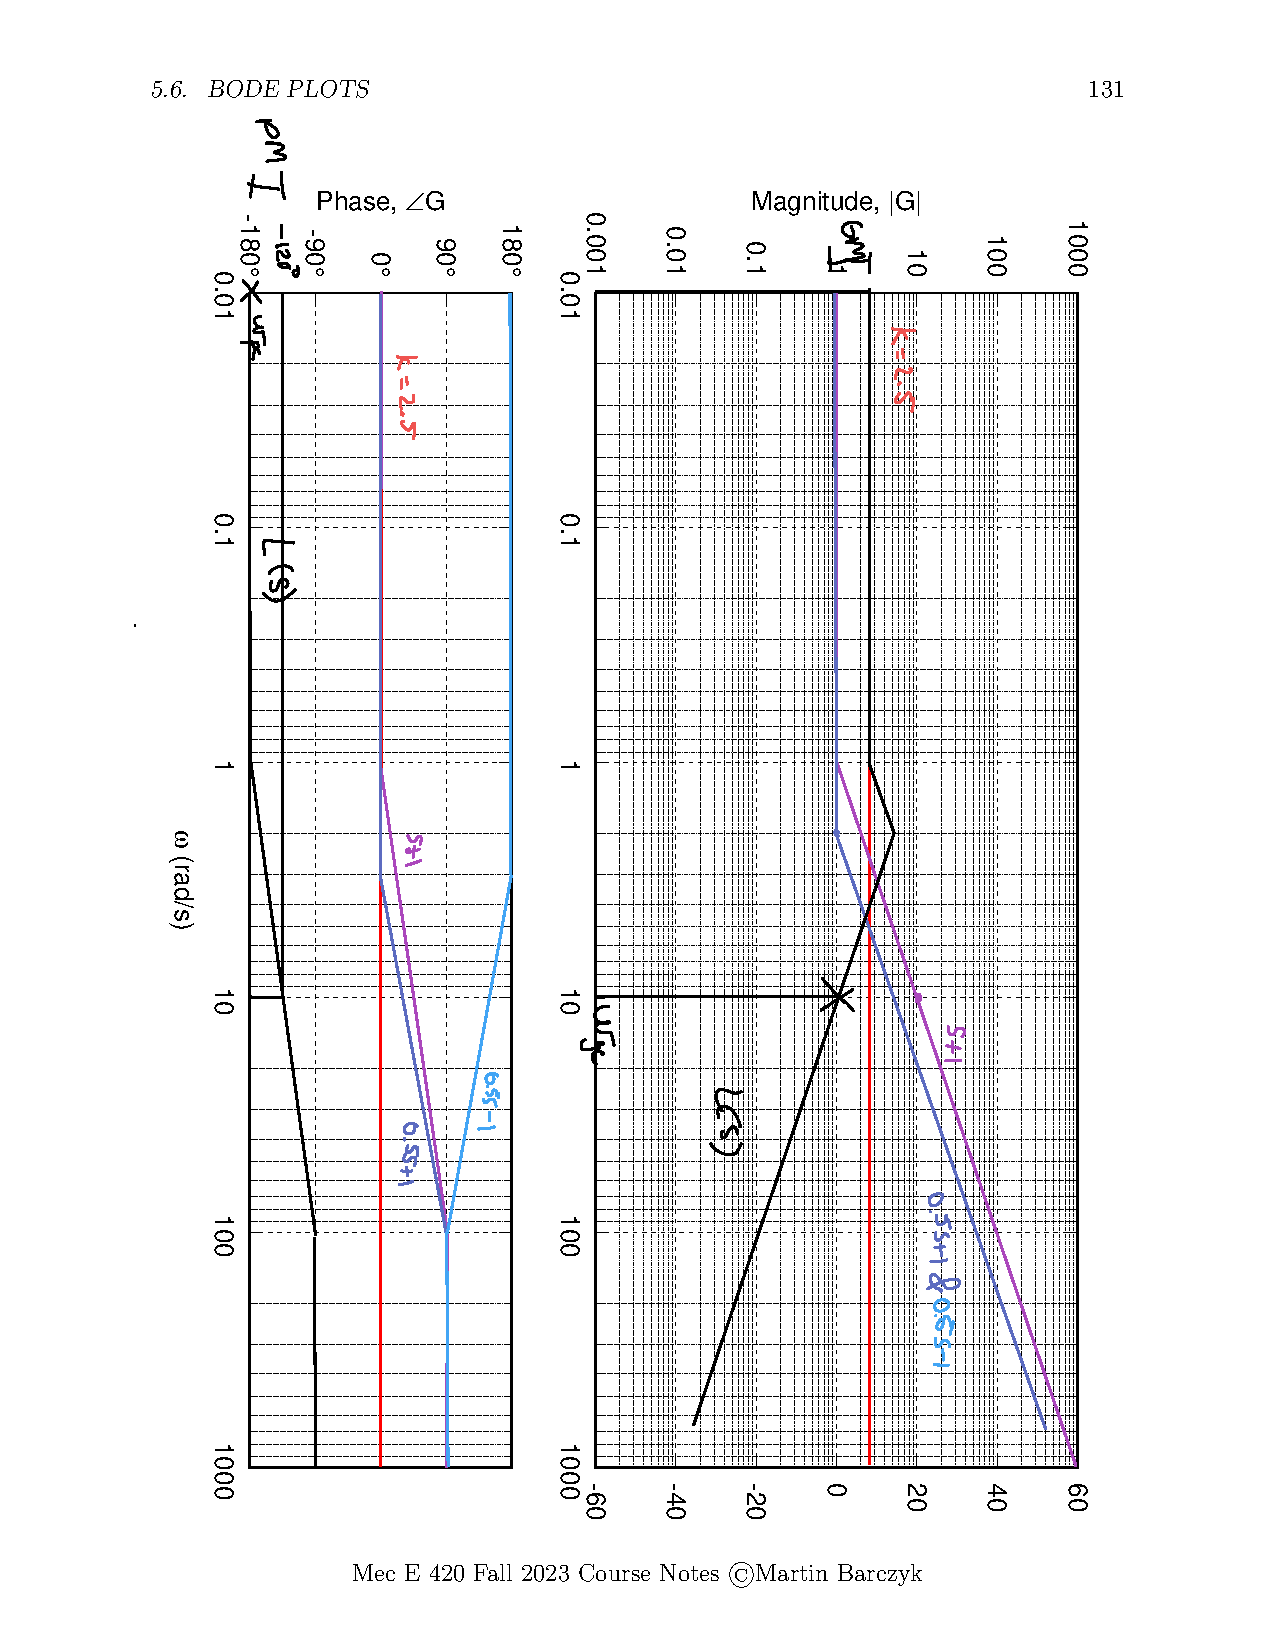
\includepdf[]{Q2 sketch.pdf}

\begin{itemize}
    \item $\omega_{\text{gc}} \approx 10$
    \item $\omega_{\text{pc}} = 0$
    \item Gm $=1/2.5 = 0.4$
    \item Pm $\approx 60^\circ$
\end{itemize}
\subsection{}
\textit{Use MATLAB’s margin command to validate your results from (a) and (b). Include a print-out
of the resulting plot}
By Matlab,
\begin{lstlisting}[language=Matlab]
syms s
L = 2.5*(s+1)/((0.5*s-1)*(0.5*s+1));
[n, d] = numden(L);
n = sym2poly(n);
d = sym2poly(d);
margin(tf(n, d));
\end{lstlisting}
\begin{figure}[h]
    \centering
    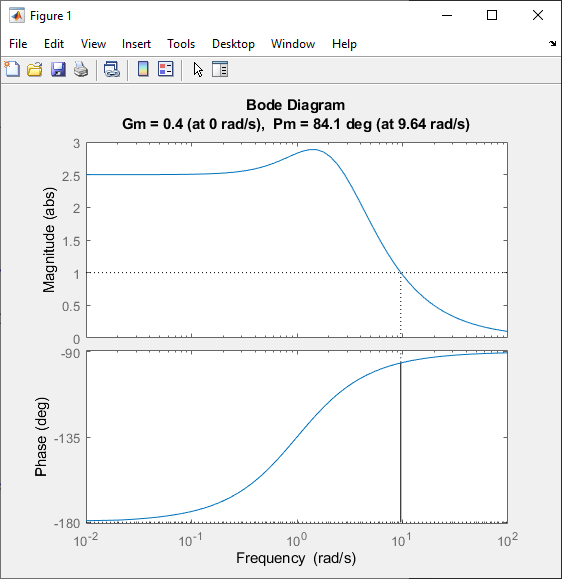
\includegraphics[width=0.5\linewidth]{Questions/Figures/Q2 Matlab Margin.png}
    \caption{Margin plot of $L(s)$ using Matlab}
    \label{fig:Q2 Matlab Margin}
\end{figure}
From the plot,
\begin{itemize}
    \item $\omega_{\text{gc}} = 9.64$
    \item $\omega_{\text{pc}} = 0$
    \item Gm $=0.4$
    \item Pm $=84.1^\circ$
\end{itemize}

\subsection{}
\textit{Using the values identified in (c), calculate the delay margin $t_{d}^{\text{max}}$ for this closed-loop system}
\begin{align*}
    t_{d}^{\text{max}} = \frac{\text{PM}}{\omega_{\text{gc}}} = \frac{84.1\times \frac{\pi}{180}}{9.64} = 0.152 \text{ s}
\end{align*}

\subsection{}
\textit{Calculate the Nyquist Margin NM of this design (give the MATLAB commands you used)}
By Matlab,
\begin{lstlisting}[language=Matlab]
syms s
L = 2.5*(s+1)/((0.5*s-1)*(0.5*s+1));
[n, d] = numden(L);
n = sym2poly(n);
d = sym2poly(d);

bodemag(tf(n, d));
\end{lstlisting}

\begin{figure}[h]
    \centering
    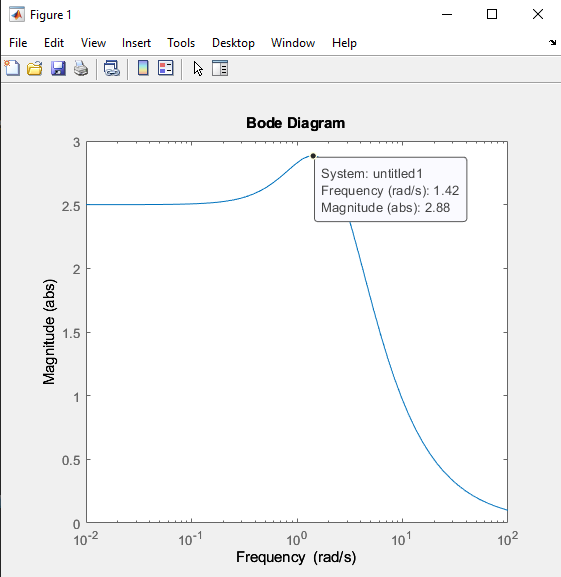
\includegraphics[width=0.5\linewidth]{Questions/Figures/Q2 Matlab Bodemag.png}
    \caption{Bode magnitude plot of $L(s)$ using Matlab}
    \label{fig:Q2 Matlab BodeMag}
\end{figure}

On the plot, the peak is 2.88. Therefore, $\boxed{\text{NM} = 1/2.88 = 0.347}$.

